\chapter{Implementation} \label{chap:impl}

This chapter provides a detailed description of the implemented system. In Section~\ref{sec:impl-GM}, the Geometric Monitoring method implementation is described, along with the necessary simplifying assumptions to aid experimentation. Following that, in Section~\ref{sec:impl-distNodeMatch} an algorithm for node matching is proposed, inspired by the violation recovery method found in~\cite{Keren2014GMHetStreams}. In Section~\ref{sec:impl-heuristic}, the heuristic based balancing method for local violation resolution is presented, along with the necessary data stream tracking scheme. Finally, the main implementation challenges are discussed.

\section{Geometric Monitoring Implementation} \label{sec:impl-GM}

The initial Geometric Monitoring method~\cite{Sharfman2006GM}, which is described in detail in Section~\ref{sec:theorBack-GM}, provides two algorithms for threshold monitoring of distributed data streams. These algorithms operate on different network structures and implement a somewhat different handling of threshold violations.

The decentralized algorithm operates on a coordinator-less environment, where nodes are allowed to communicate with each other, whereas the coordinator-based algorithm has a Star network topology, where the coordinator node is the central node (the \emph{hub}) and the Monitoring nodes reside on the edges of the network.
The algorithm operating on the decentralized setting does not provide a balancing process for local violation resolution. On the other hand, the coordinator based algorithm implements a violation resolution operation every time a local violation occurs, which aims to minimize the communication overhead induced by false violation reports. 

Our focus is centered towards a simplified \textbf{coordinator-based algorithm} (Algorithms~\ref{algo:centralizedCoordinatorNode},  and~\ref{algo:centralizedMonitoringNode}), described in Section~\ref{sec:theorBack-GM}, as it provides a framework for the heuristic balancing process, as well as the node matching operation presented in detail in Sections~\ref{sec:impl-heuristic} and~\ref{sec:impl-distNodeMatch} respectively.

To aid method formulation and experimentation, the following simplifying assumptions have been made regarding the coordinator-based algorithm:
\begin{itemize}
\item Communication between nodes is considered instantaneous. There is no delay when passing messages through the network. The problem of message handling in a real-world Geometric Monitoring method implementation, where message delays are induced by the underlying network, has been studied in detail in~\cite{Babis2013SimulatorStreams}.

\item Communication between nodes is considered loss-less and reliable. In case network reliability can not be guaranteed appropriate methods should be considered.

\item The system operates in an iterative fashion, as described in Algorithm~\ref{algo:singleHandlingNetwork}. This simplification of the real-time distributed monitoring process to an iterative process provides a more manageable setting for experimentation without distorting the results of the proposed methods, which can be applied directly to the original real-time distributed setting.

\item The system pauses at each violation, until the violation is resolved. During violation resolution Monitoring nodes do not receive updates from their respective data streams.

\item The Coordinator node does not participate in the monitoring operation. The Coordinator node does not receive updates from a data stream, it only receives messages from the Monitoring nodes in case of threshold violation. This assumption can easily be elevated by considering an additional monitoring node responsible for handling the coordinator's data stream monitoring operation. 

\end{itemize}

%TODO: mention training and testing dataset?
%TODO: implementation specifics, ball computation (i.e. optimization)?

%%%%%%%%%%%%%%%%%%%%%%%%%%%%%%%%%%%%%%%% single handling network algo %%%%%%%%%%%%%%%%%%%%%%%%%%%%%%%%%%%%%%%%%%%
\begin{algorithm}[H]
\setstretch{1.30}

\KwData{$monitoringNodes$: a list of Monitoring nodes,~$coordinator$: the Coordinator node}

\SetAlgoLined
\Begin{
 initialization\;
 	\Repeat{$globalViolation$}{
		\ForEach{$node \in\ monitoringNodes$}{
			$node.DataVectorUpdate()$\;
			$node.ComputeDriftVector()$\;
		}
		\ForEach{$node \in\ monitoringNodes$}{
			$node.CheckForViolation()$\;
			\If{$localViolation$}{
				$node.Report()$\;
				$coordinator.Balance()$\;
			}
		}
	}
}
\caption{Iterative network operation \label{algo:singleHandlingNetwork}} 
\end{algorithm}
%%%%%%%%%%%%%%%%%%%%%%%%%%%%%%%%%%%%%%%%%%%%%%%%%%%%%%%%%%%%%%%%%%%%%%%%%%%%%%%%%%%%%%%%%%%%%%%%%%%%%%%%%%%%%%%

\section{Distance Based Node Matching} \label{sec:impl-distNodeMatch}
%TODO: check my notes for things to add

The balancing method of the coordinator-based algorithm, as described in Section~\ref{sec:theorBack-GM}~\cite{Sharfman2006GM, Sharfman2012ShapeSensGM}, aims at resolving local violations that do not result in a global violation (\emph{false alarms}) by balancing the violating node's drift vector with the respective vectors of \emph{randomly} chosen nodes. Consider the violating node $n_i$ with weight $w_i=1$, so that the bounding ball $B(\vec{e}(t), \vec{u_i}(t))$ is not monochromatic, and the randomly requested node $n_j$ with weight $w_j=1$, so that the newly formed bounding ball is $B(\vec{e}(t), \frac{\vec{u_i}(t)+\vec{u_j}(t)}{2})$, where $\vec{e}(t)$ the estimate vector at time $t$ and $\vec{u_i}(t)$, $\vec{u_j}(t)$ the drift vectors of nodes $n_i$, $n_j$ at time $t$, respectively. If the resulting bounding ball is monochromatic the violation is resolved, otherwise another node is \emph{randomly} requested for balancing.

As observed in~\cite{Keren2014GMHetStreams, BenDavid2012ViolationRI}, the original balancing method's node choosing scheme can be inefficient, so a more efficient and deterministic approach should be adopted. Optimal pairing of nodes and the construction of a hierarchical structure (Figure~\ref{fig:nodePairHierarchy}) reduces the communication overhead of false alarms, with the vast majority of violation resolutions requiring only the assigned node pair to be successful. The criterion by which nodes are paired attempts to maximize the probability of a successful balance by maximizing \textit{``the percentage of pairs of data vectors from both nodes whose sum is in the Minkowski sum of the nodes' safe-zones''}~\cite{Keren2014GMHetStreams}, or, in this case, whose resulting bounding ball is monochromatic.

Here, the same node pairing scheme is followed, but with a different, distance based, criterion for grouping nodes into disjoint pairs and creating the hierarchical structure depicted in Figure~\ref{fig:nodePairHierarchy}. The method proceeds as follows (Algorithm~\ref{algo:nodeMatching}):
\begin{enumerate}
\item Monitoring nodes are visualized as the nodes of a complete graph $G=(V,E)$, where $V=\{n_1, n_2, ... , n_k\}$ vertex set consists of the initial Monitoring nodes (\emph{``Type-1 nodes''}) and $E=\{(n_i, n_j)\ \forall i,j \in [1, ..., k], i \neq j\}$ edge set contains an edge for every pair of vertices.
\item Weights are assigned to all edges $E$. The weight of each edge is defined as the cumulative distance of the value of the monitoring function on the mean of each pair of data vectors from the value of the monitoring function on the \emph{global} mean of all Monitoring nodes' data vectors, plus the cumulative distance of each pair of data vectors:
\begin{equation}
w_{i,j}=
\sum_{t=t_0}^{t_{end}}{[(f(\vec{v}_{global}(t))-f(\frac{\vec{v_i}(t)+\vec{v_j}(t)}{2}))+(|\vec{v_i}(t)-\vec{v_j}(t)|)]}
\label{form:distanceMatchingWeights}
\end{equation}
, where $\vec{v_i}(t)$ the data update of node $n_i$ at time $t$, $\vec{v}_{global}(t)$ the global mean of all Monitoring nodes at time $t$ and $f(\cdot)$ the monitoring function.

\item Maximum weighted matching is performed on the resulting graph via the \emph{primal-dual} method implemented in the \emph{networkx} Python library~\cite{networkxMaxWeight}, so that nodes are partitioned into disjointed sets $M_i$, $|M_i|=2\ \forall i \in [1, ..., \frac{k}{2}]$. 

\item Each set $M_i, i \in [1, ..., \frac{k}{2}]$ is considered a single node, so that a new complete graph $G'=(V', E')$ is created, where $V'=\{M_1, ..., M_{\frac{k}{2}}\}$ (\emph{``Type-2 nodes''}) the new vertex set and $E'=\{(M_i, M_j)\ \forall i,j \in [1, ..., \frac{k}{2}]\}$ the new edge set. Weights are assigned to the new edges and the process repeats until the resulting graph contains only a single vertex (\emph{``Type-k node''}), which incorporates all the initial Monitoring nodes.

\item Vertices not matched with any other vertex during the matching process are ignored in future iterations. During the balancing process such unmatched vertices are handled by the traditional random selection balancing algorithm found in~\cite{Sharfman2006GM}(also, Section~\ref{sec:impl-GM}). 
\end{enumerate} 
~
%%%%%%%%%%%%%%%%%%%%%%%%%%%%%%%%%%%% hierarchy figure %%%%%%%%%%%%%%%%%%%%%%%%%%%%%%%%%%%%
\begin{figure}
\centering
\includegraphics[trim=0 9cm 0 0]{img/NodeMatchingHierarchy.tex}
\caption{Hierarchical pairing scheme example  for node set $\{n_1, n_2, n_3, n_4, n_5, n_6, n_7, n_8\}$.} 
\label{fig:nodePairHierarchy}
\end{figure}
%%%%%%%%%%%%%%%%%%%%%%%%%%%%%%%%%%%%%%%%%%%%%%%%%%%%%%%%%%%%%%%%%%%%%%%%%%%%%%%%%%%%%%%%%%%

%%%%%%%%%%%%%%%%%%%%%%%%%%%%%%%%%%%% node matching algo %%%%%%%%%%%%%%%%%%%%%%%%%%%%%%%%%%%
\begin{algorithm}[H]
\SetAlgoLined
\setstretch{1.30}
\SetKwFunction{DistancePairer}{DistancePairer}
\SetKwProg{Fn}{Function}{}{end}
\Fn{\DistancePairer{$nodes$,$i$}}{
	\KwData{$nodes=[(n_1, [\vec{v_1}(t_0), ... , \vec{v_1}(t_{end})]), ... , (n_k, [\vec{v_k}(t_0), ... , \vec{v_k}(t_{end})])]$: list of nodes with their respective data vectors,$i$: pair type, initial=1} 
	\KwResult{$nodeHierarchy$: dictionary of \emph{Type-k} pairs}

	\If(\tcp*[f]{recursion stopping condition}){$length(nodes)=1$}{
		\Return{$nodeHierarchy$}\;
	}
	$g=CreateCompleteGraph(nodes)$\tcp*[r]{complete graph with $nodes$ as vertices} 
	\ForEach(\tcp*[f]{assign weights to edges}){$(n_i, n_j)\in g.Edges()$}{
		$w_{i,j}=
		\sum_{t=t_0}^{t_{end}}{[(f(\vec{v}_{global}(t))-f(\frac{\vec{v_i}(t)+\vec{v_j}(t)}{2}))+(|\vec{v_i}(t)-\vec{v_j}(t)|)]}$\;
		$g.edge(n_i, n_j).weight=w_{i,j}$\;
	}
	$nodeHierarchy(\text{Type-i})=g.maximalWeightMatching()$\tcp*[r]{node pairs of \emph{Type-}$i$}
	\DistancePairer{$nodeHierarchy(\text{Type-i}),i*2$}\;
}
\caption{Recursively create Monitoring node pairs and hierarchy \label{algo:nodeMatching}} 
\end{algorithm}
%%%%%%%%%%%%%%%%%%%%%%%%%%%%%%%%%%%%%%%%%%%%%%%%%%%%%%%%%%%%%%%%%%%%%%%%%%%%%%%%%%%%%%%%%%%
~
%%%%%%%%%%%%%%%%%%%%%%%%%%%%%%%%%%%% distance figure %%%%%%%%%%%%%%%%%%%%%%%%%%%%%%%%%%%%    
\begin{figure}
        \centering
		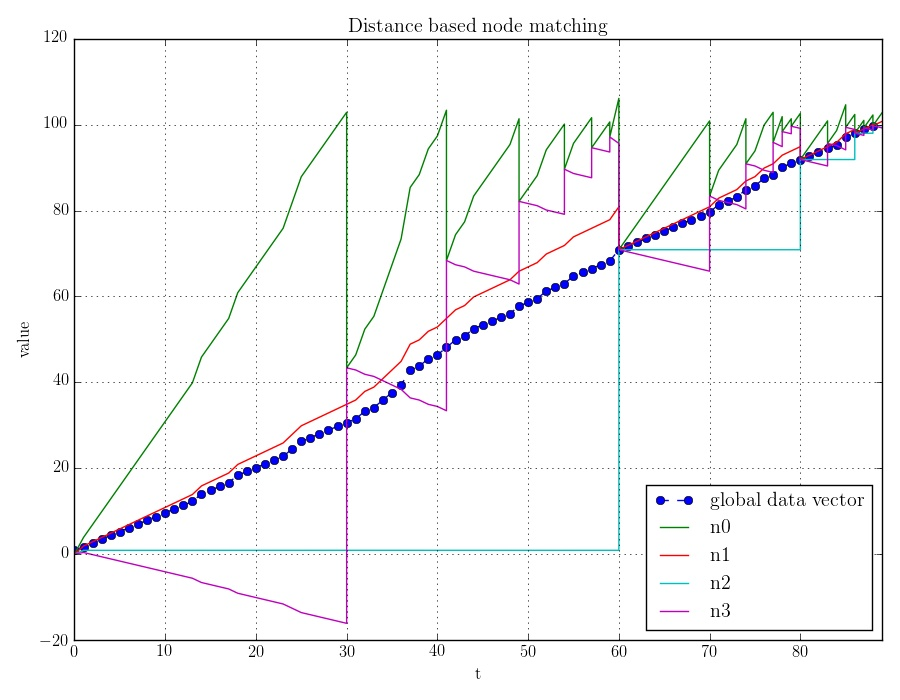
\includegraphics[scale=0.30]{img/distoptpair_example_full.jpeg}
        \caption{The drift vectors during Geometric Monitoring operation until a Global Violation. Distance based node matching is used on 4 nodes ($\{n_0, n_1, n_2, n_3\}$), with 1-dimensional data vectors, threshold $T=100$ and $f(x)=x$ as the monitoring function. The \emph{Type-2} node pairs are $\{n_0, n_3\}$ and $\{n_1, n_2\}$.}\label{fig:distoptpair}
\end{figure}
\begin{figure}
        \centering
		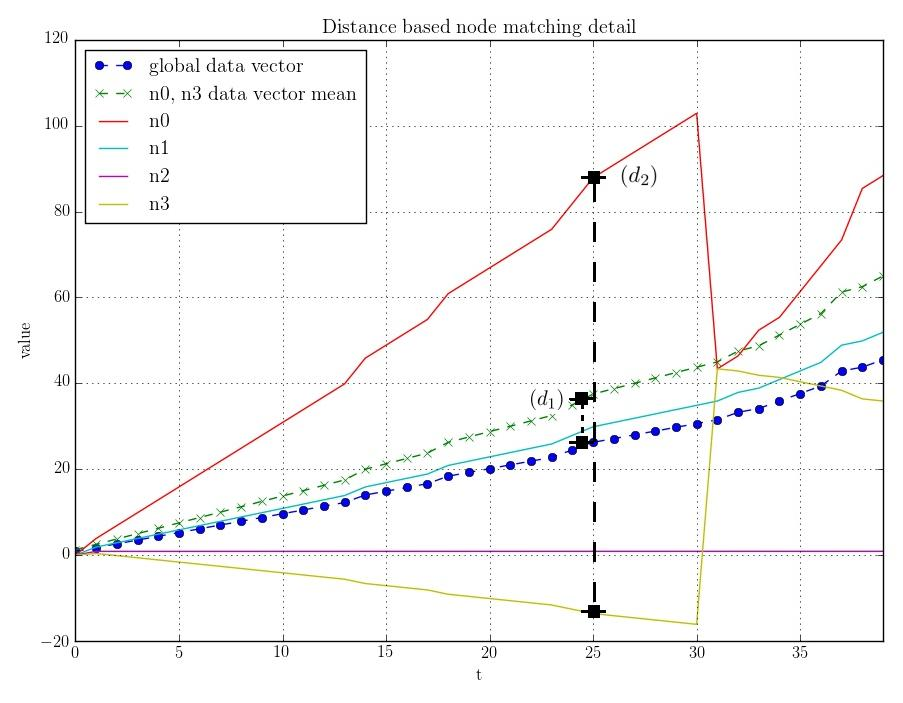
\includegraphics[scale=0.30]{img/distoptpair_example_detail_edited.jpeg}
        \caption{Detailed depiction of the Geometric Monitoring operation of Figure~\ref{fig:distoptpair}. Distance based node matching operating on 4 nodes ($\{n_0, n_1, n_2, n_3\}$), with 1-dimensional data vectors, threshold $T=100$ and $f(x)=x$ as the monitoring function. Distance $d_1$ denotes the distance of the data vector mean of the paired nodes $n_0$ and $n_3$ from the global mean (\emph{global data vector}) at $t=25$, whereas distance $d_2$ denotes the in-between distance of data vectors $\vec{v_0}(t)$ and $\vec{v_3}(t)$ of the node pair at time $t=25$ (before a Local Violation occurs, where $\vec{e}=0$ and $\vec{u_i}(t)=\vec{v_i}(t)\ \forall\ i\in[0,1,2,3], t<30$). Both distances are taking part in the edge weighting process, according to Equation~\ref{form:distanceMatchingWeights}.} \label{fig:distoptpairdetailed}
\end{figure}%
%%%%%%%%%%%%%%%%%%%%%%%%%%%%%%%%%%%%%%%%%%%%%%%%%%%%%%%%%%%%%%%%%%%%%%%%%%%%%%%%%%%%%%%%%%%

The incentive behind the distance based node pairing scheme comes from the need to track the global data vector as closely as possible, with only a subset of the total node population's data vectors at each balancing attempt. By considering the distance of the mean of a pair of data vectors from the global data vector (distance $d_1$ in Figure~\ref{fig:distoptpairdetailed}) the \emph{``quality''} and \emph{``accuracy''} of the tracking ability of each pair is evaluated. Additionally, by taking into account the in-between distance of data vectors of each node pair (distance $d_2$ in Figure~\ref{fig:distoptpairdetailed}), pairs from the limits of the data vector velocity spectrum that manage to \emph{``cancel each other out''} more effectively are encouraged.

\section{Heuristic Balancing} \label{sec:impl-heuristic}
%TODO: check notes for additional stuff to add

The balancing method incorporated into the \emph{coordinator based} algorithm of the Geometric Monitoring method~\cite{Sharfman2006GM} (Section~\ref{sec:theorBack-GM}) attempts to minimize the communication overhead of local violations by computing the, so called, \emph{balancing vector}. The \emph{balancing vector} is defined as the weighted mean of the drift vectors of the nodes contained in the balancing set, and, in case of a successful balance, it is guaranteed that $B(\vec{e}, \vec{b})$ is monochromatic. Consequently, by setting the drift vectors of the nodes in the balancing set to be equal to the balance vector, all local constraints are fulfilled and the convexity property of the drift vectors is satisfied.

While this method partially succeeds in reducing the communication burden of false alarms either by requesting only a subset of the total node set each time a Local Violation occurs or by setting the drift vectors to a safe point (represented by the balance vector), major drawbacks can be noted regarding vector positioning and bounding ball construction. Updated vector assignment as a result of the ``optimization'' procedure does not take into account the idiosyncrasies of the monitoring function and the admissible region it produces. Additionally, all nodes taking part in the balancing process are handled identically, without taking advantage of the differences in the behavior of each node.

Previous work proposed selecting an optimal reference vector, instead of the estimate vector for bounding ball construction, along with shape customization of the local constraints at the nodes according to the node's needs~\cite{Sharfman2012ShapeSensGM}. Local constraint customization served as the basis for the now popular \emph{Safe-Zone} framework~\cite{Keren2013SafeZones, Keren2014GMHetStreams}, which diverges from the traditional bounding sphere setting, while maintaining the same fundamental idea of distance computation of a point from a set of support vectors~\cite{Samoladas2013Unification}, preserving the essence of the admissible region and retaining the balancing process of the coordinator based scenario.

This thesis proposes a novel heuristic approach for optimal positioning of drift vectors, which takes into account both the temporal behavior of each node's data stream, as well as the peculiarities of the monitoring function over said data streams. Aim of the heuristic optimization is the maximization of the estimated time until the following Local Violation occurs, which, expressed as an optimization formula, receives the following form:
\begin{equation}
\max\min \frac{(T-x_i)-accel_i(t_{lv})*t^2}{vel_i(t_{lv})}, \forall n_i \in P'
\label{form:heuristic}
\end{equation}
where:
\begin{align*}
t&:\text{the variable to optimize}\\
T&:\text{monitoring threshold}\\
x_i&:\text{the maximum value of the monitoring function $f(\cdot)$ over the bounding ball $B(\vec{e}(t_{lv}), \vec{u_i}(t_{lv}))$,}\\&\qquad\text{where $t_{lv}$ is the time a Local Violation occurred and $i$ the index of node $n_i$}\\
vel_i(t_{lv})&:\text{the estimated velocity of the maximum value of the monitoring function $f(\cdot)$}\\&\qquad\text{when applied to the bounding ball created by the data stream update of node $n_i$}\\&\qquad\text{and the estimate vector $\vec{e}$ at time $t_{lv}$}\\
accel_i(t_{lv})&:\text{the estimated acceleration of the maximum value of the monitoring function $f(\cdot)$}\\&\qquad\text{when applied to the bounding ball created by the data stream update of node $n_i$}\\&\qquad\text{and the estimate vector $\vec{e}$ at time $t_{lv}$}\\
t_{lv}&:\text{time of Local Violation occurrence}\\
P'&:\text{the balancing set}\\
\end{align*}

The Equation~\ref{form:heuristic} originates from elementary kinematic equations, as such:\\
Assume a moving object $i$ at point $x_i$, with acceleration $a_i$ and current velocity $v_i$. Let $v_f$ be the object's final velocity when it reaches a threshold point $T$ at time $t$, from which it deviates by $d=T-x_i$. Let current time be $t=0$.\\
Distance (or \emph{Displacement}) in terms of velocity and acceleration is described by:
\begin{equation}
d=v_i t+a t^2
\label{form:displacement}
\end{equation}
For which it holds:
\begin{align*}
d&=v_i t+a_i t^2 \leftrightarrow\\
T-x_i&=v_i t + a_i t^2 \leftrightarrow\\
t&=\frac{(T-x_i)-a_i t^2}{v_i}\\
\end{align*}
Thus, $t$ is the expected time the moving object reaches the threshold point $T$.

The newly defined heuristic optimization formula (\ref{form:heuristic}) aims to maximize the time until the next Local Violation concerning any of the nodes belonging in the balancing set. By taking into account the maximum value of the monitoring function $f(\cdot)$ inside the bounding ball created by each data stream update and the estimate vector, and by computing acceleration and velocity measures of this value over time, an approximate mapping of the data stream space to the one dimensional space of the arbitrary monitoring function is achieved. This permits the computation of the optimal positions the balanced drift vectors should take in order to maximize the time they reach the monitoring threshold, as depicted in Figure~\ref{fig:heuristicbalancing}.

%%%%%%%%%%%%%%%%%%%%%%%%%%%%%%%%%%%% balancing figure %%%%%%%%%%%%%%%%%%%%%%%%%%%%%%%%%%%%
\begin{figure*}[t!]
\centering
\begin{subfigure}[t]{0.45\textwidth}
\centering
\includegraphics[scale=0.45]{img/classic_balancing.tex}
\caption{The classic balancing method. As long as $B(\vec{e}, \vec{b})$ is monochromatic (i.e. within the Admissible region), balance is successful and the updated drift vectors are set to $\vec{u_1}'=\vec{u_2}'=\vec{b}$.} 
\label{fig:classicbalancing}
\end{subfigure}
\begin{subfigure}[t]{0.45\textwidth}
\centering
\includegraphics[scale=0.45]{img/heuristic_balancing.tex}
\caption{The heuristic balancing method. Arrows depict the velocities of each drift vector. After a successful balance is achieved ($B(\vec{e}, \vec{b})$ is monochromatic), the optimal points in which the updated drift vectors ($\vec{u_1}', \vec{u_2}'$) should be positioned are computed by maximizing the estimated time until the next Local Violation, based on the current drift vector positions and the estimated velocities. Balance vector $\vec{b}$ remains unchanged.\\} 
\label{fig:heuristicbalancing}
\end{subfigure}
\caption{Balancing methods}
\end{figure*}
%%%%%%%%%%%%%%%%%%%%%%%%%%%%%%%%%%%%%%%%%%%%%%%%%%%%%%%%%%%%%%%%%%%%%%%%%%%%%%%%%%%%%%%%%%%

\subsection{Implementation of the Heuristic Balancing}

%TODO: include relaxing of threshold
In order transform the heuristic optimization formula (\ref{form:heuristic}) into an applicable setting, \emph{multi-objective optimization} (Section~\ref{sec:theorBack-MOP}) is used. The optimization function is now defined as such:
\begin{align*}
\min -z&\\
	\text{s.t.}\ \ z&\leq g(h(\vec{e},\vec{u_0}), vel_0, accel_0, T)\\
	z&\leq g(h(\vec{e},\vec{u_1}), vel_1, accel_1, T)\\
	&\vdots  \numberthis \label{form:mop}\\
	z&\leq g(h(\vec{e},\vec{u_n}), vel_n, accel_n, T)\\
	\vec{b}&=\frac{1}{\sum_{i=0}^n{w_i}}\sum_{i=0}^n{(w_i*\vec{u_i})} &&,\forall n_i \in P'
\end{align*}
where:
\begin{align*}
g&:\mathbb{R}^4 \to \mathbb{R}, \text{the heuristic optimization function as defined in Equation~\ref{form:heuristic}}\\
h&:\mathbb{R}^d \to \mathbb{R}, \text{the function computing the maximum value of the monitoring function $f(\cdot)$ in $B(\vec{e},\vec{u_i})$,}\\&\qquad\text{which is an optimization problem by itself}\\
d&: \text{the data vector dimensionality}\\
T&: \text{the monitoring threshold}\\
\vec{u_i}&: \text{the drift vector of node $n_i$}\\
w_i&: \text{the weight of node $n_i$}\\
vel_i&: \text{the velocity of the maximum value of the monitoring function when applied to the ball}\\&\qquad\text{ defined by node's $n_i$ drift vector $\vec{u_i}$ and the estimate vector $\vec{e}$}\\
accel_i&: \text{the acceleration of the maximum value of the monitoring function when applied to the ball}\\&\qquad\text{ defined by node's $n_i$ drift vector $\vec{u_i}$ and the estimate vector $\vec{e}$}\\
\vec{b}&: \text{the balancing vector}\\
P'&: \text{the balancing set}
\end{align*}
\newpage
Solution to the above optimization problem (\ref{form:mop}) is given by a \emph{Sequential Least Squares Programming (SLSQP)} solver, which implements \emph{sequential quadratic programming} (described briefly in Section~\ref{subsec:theorBack-NCOP}) by using the \emph{Han-Powell quasi-Newton} method with \emph{BFGS} update at each iteration for the Hessian matrix approximation, and an \emph{L1-test function} for computing the step length. The solver is implemented by the \emph{pyOpt} Python optimization library~\cite{pyOptSLSQP}. The problem is decomposed and formulated using an additional helping parameter $z$ in order to avoid non-differentiable functions (such as $\min$ and $\max$) and to aid computation by the solver.

In the heuristic optimization problem defined previously (\ref{form:mop}) the nested optimization of detecting the maximum value of an arbitrary monitoring function inside the bounding ball $B(\vec{e},\vec{u_i})$ is existent. This optimization problem is formed as follows:
\begin{align}
\max &\quad f \label{form:maxvalinball-func}\\
	\text{s.t.}&\quad \sum_{i=1}^d(x_i-c_i)^2=r^2 \label{form:maxvalinball-ball}
\end{align}
where:
\begin{align*}
f&: \text{the monitoring function $f(\cdot)$}\\
x_i&: \text{element $i$ of $d$-dimensional vector $\vec{x}$}\\
c_i&: \text{element $i$ of $d$-dimensional vector $\vec{c}$, which represents the center of the sphere}\\
r&: \text{the radius of the sphere}\\
d&: \text{the space dimensionality}\\
\text{Eq.~\ref{form:maxvalinball-ball}}&:\text{a $(d+1)$ dimensional sphere in $\mathbb{R}^d$}
\end{align*}

The optimization problem of detecting the maximum value of a function inside a sphere (\ref{form:maxvalinball-func}) is solved using \emph{Constrained Function Minimization (CONMIN)}, which implements the method of feasible directions, as described in Section~\ref{subsec:theorBack-NCOP} and implemented by the \emph{pyOpt} Python optimization library~\cite{pyOptCONMIN}.
\newpage
The resulting heuristic balancing algorithmic implementation is summarized in the following Algorithm:\\
%%%%%%%%%%%%%%%%%%%%%%%%%%%%%%%%%%%% node matching algo %%%%%%%%%%%%%%%%%%%%%%%%%%%%%%%%%%%
\begin{algorithm}[H]
\SetAlgoLined
\setstretch{1.30}
\SetKwFunction{RepMessageReceived}{RepMessageReceived}
\SetKwFunction{RequestNode}{RequestNode}
\SetKwFunction{Balance}{Balance}
\SetKwProg{Fn}{Function}{}{end}

\Fn{\RepMessageReceived{$<n_i$,$v_i$,$u_i$,$vel_i$,$accel_i>$}}{
	add $n_i$ to balancing set $P'$\;
	\Balance{}\;
}

\Fn{\Balance{$P'$}}{
	\If{$length(P')=1$}{
		\RequestNode{}\tcp*[r]{request node based on respective gathering scheme}
	}

	$\vec{b}=\sum_{P'}{\frac{w_i*\vec{u_i}}{w_i}}$\;

	\If{$B(\vec{e},\vec{b})$ is monochromatic}{
		\tcc{heuristic optimization procedure,\\ returns the optimal drift vector positions in set $O$}
		$O=DriftVectorOptimizationProblem()$\;

		\ForEach{$n_i \in P'$}{
			$\Delta\delta_i=w_i*\vec{u_i}'-w_i*\vec{u_i}$\tcp*[r]{$\vec{u_i}'$ denotes the optimal drift vector position}
			$Send(<ADJSLK,n_i,\Delta\delta_i>)$\;
		}
	}
}
\caption{Heuristic Balancing \label{algo:heuristicbalancing}} 
\end{algorithm}
%%%%%%%%%%%%%%%%%%%%%%%%%%%%%%%%%%%%%%%%%%%%%%%%%%%%%%%%%%%%%%%%%%%%%%%%%%%%%%%%%%%%%%%%%%%

\subsection{Smoothing, Velocity and Acceleration Estimation via Savitzky-Golay} \label{subsec:impl-heuristic-vel}

The heuristic balancing method proposed previously (Section~\ref{sec:impl-heuristic}) requires an efficient estimation of the velocity and the acceleration of the output of the monitoring function over the maximum value of the bounding ball. Additionally, a smoothing operation over the data stream series would be beneficial, in order to grasp the trend (increasing or decreasing) of the data stream without letting noisy updates and extreme fluctuations misguide the optimization operation. 

The \emph{Savitzky-Golay smoothing filter}~\cite{SavGol1964SmoothDiff} (Section~\ref{sec:theorBack-SavitzkyGolay}) is ideal in the heuristic Geometric Monitoring setting, for it smooths and derivates the signal without much additional computational burden, allowing it to be applied directly at the Monitoring Nodes' data streams. By assuming equidistant data points the precomputation of convolution coefficients becomes trivial when specifying the window size, the window center, the order of the polynomial and the desired derivative. Following that, the precomputed coefficients are applied to the desired signal by a simple convolution, which is both fast and, if required, on-line. The application of the filter on a noisy signal, along with the velocity and the acceleration computation of this signal, is shown in Figure~\ref{fig:savgol}.


%%%%%%%%%%%%%%%%%%%%%%%%%%%%%%%%%%%% savgol figure %%%%%%%%%%%%%%%%%%%%%%%%%%%%%%%%%%%
\begin{figure}
\centering
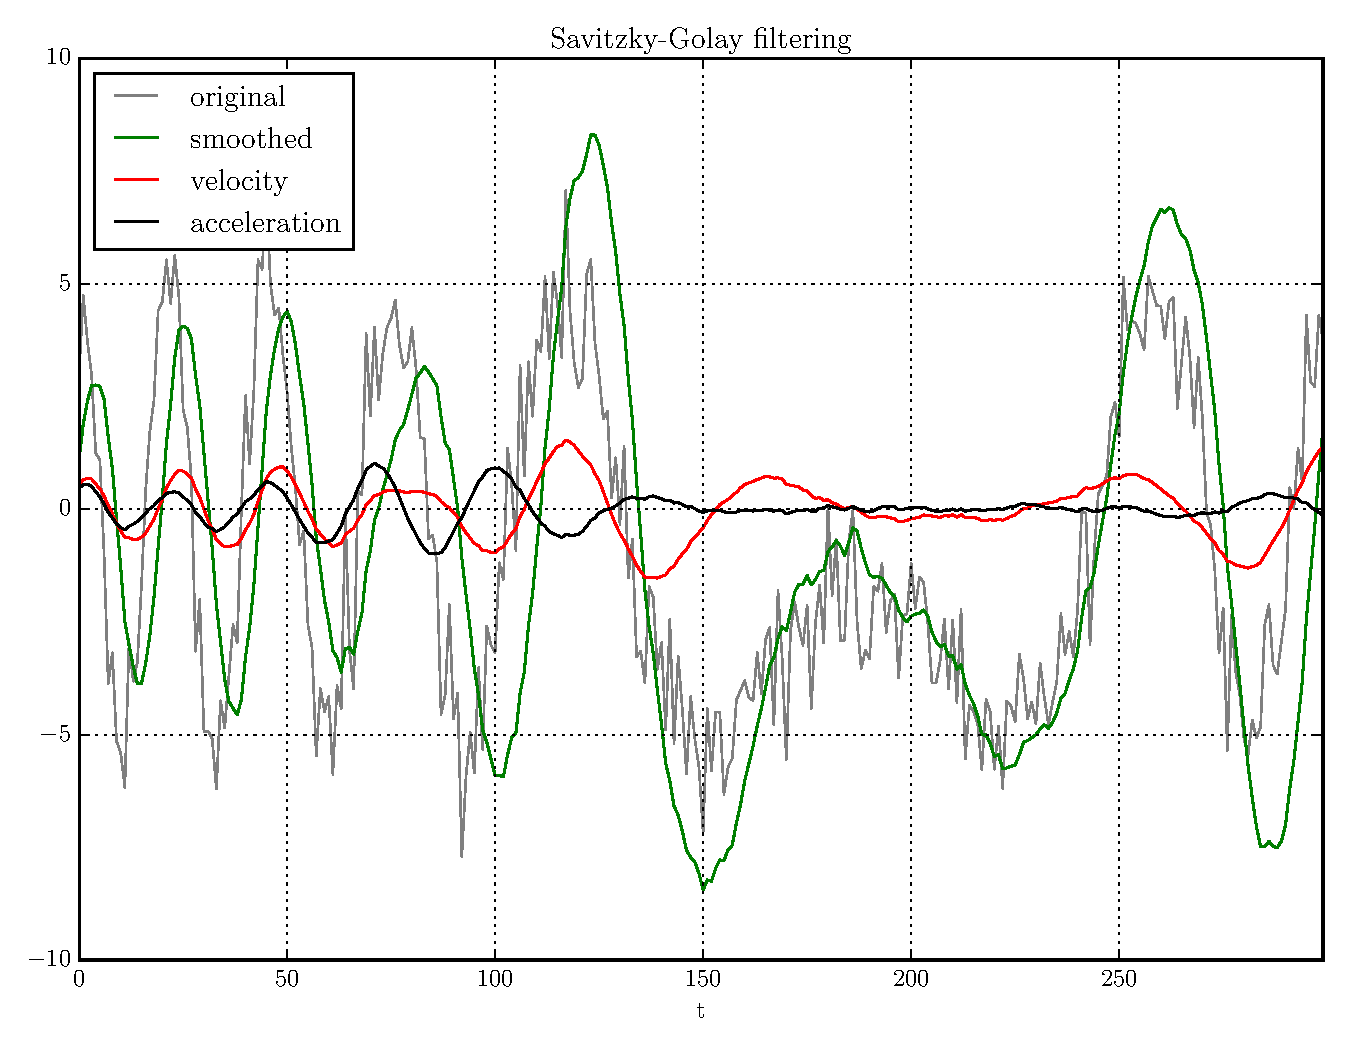
\includegraphics[scale=0.60]{img/savgol.pdf}
\caption{Savitzky-Golay filtering of a signal with added Gaussian noise. The smoothing window is 50 points in length, centered at the far end, as in the real-time smoothing applied to the Geometric Monitoring setting. The polynomial order is 2 for the smoothed signal, 3 for the velocity estimation and 5 for the acceleration estimation of the original signal.} 
\label{fig:savgol}
\end{figure}
%%%%%%%%%%%%%%%%%%%%%%%%%%%%%%%%%%%%%%%%%%%%%%%%%%%%%%%%%%%%%%%%%%%%%%%%%%%%%%%%%%%%%%%%%%%

\section{Implementation Challenges} \label{sec:impl-implChallenges}

The proposed methods and algorithms incur some implementation challenges, which, on the greater part, can be managed.

Regarding the \emph{distance based node matching} presented in Section~\ref{sec:impl-distNodeMatch}: 
\begin{itemize}
\item In order to extract the optimal node pairs training data must be available. This situation can be handled in two ways. One way is to initiate execution of the Geometric Monitoring task using the original method of randomly requesting nodes during balancing, until the necessary amount of data to train the model has been cumulated. Then the model can be trained and the operation can be switched to the distance based node matching scheme. A more appropriate solution could be to incrementally update the node pairs using the data provided by message passing in the standard Geometric Monitoring execution, or by occasionally polling the monitoring nodes during low network activity until a satisfiable amount of data has been gathered.
\end{itemize}

Regarding the \emph{heuristic balancing} method presented in Section~\ref{sec:impl-heuristic}:
\begin{itemize}
\item The bi-level multi-objective optimization incorporated into the method can become computationally expensive when dealing with a large balancing set or with highly dimensional data streams. Attention must be paid to the selected solvers responsible for the optimization task, for some solvers can be more effective than others in different settings and different monitoring function applications. Additionally, some solvers provide customization parameters, such as \emph{tolerance} and \emph{iteration count}, among others, that greatly influence the execution time of the optimization routine, as well as the precision of the results.
\item The \emph{Savitzky-Golay smoothing filter}, responsible for smoothing and differentiating the signals representing the maximum value of the monitoring function over the bounding spheres, is directly affected by the selected window length and the polynomial order. That being the case, care must be taken to select appropriate values that effectively track the general trends without compromising detail important to the optimization routine.
\end{itemize}